\documentclass{article}
\usepackage{graphicx}
\usepackage[latin2]{inputenc}
\usepackage{amsfonts}
\usepackage[MeX]{polski}


\title{Sprawozdanie nr 4 z Techink Programowania R�wnoleg�ego}
\author{Jakub Janczak}

\begin{document}
	\maketitle
	\section{Zadanie 1, 2, 3}
		Zadania polega�y na stworzeniu program�w przeprowadzaj�cych sumy rank�w
		\begin{enumerate}
			\item Przeprowadzaj�cy sumowanie za pomoc� funkcji reduce
			\item Przeprowadzaj�cy sumowanie cz�ciowe (za pomoc� funkcji allgather)
			\item Przeprowadzaj�cy sumowanie cz�ciowe i wypisuj�cy wyniki w kolejno�ci

			Kod �r�d�owy u autora
		\end{enumerate}

	\section{Zadania dodatkowe}
		\subsection{Broadcast}
			Celem zadania by�o zaimplementowanie programu w kt�rym jeden z proces�w wysy�a dane i odbiera od wszystkich pozosta�ych te dane z powrotem. 
		\subsection{Scatter}
			Zadanie odpowiadaj�ce, ale z u�yciem funkcji MPI\_Scatter. Nast�pnie nale�a�o por�wna� te dwie metody:

			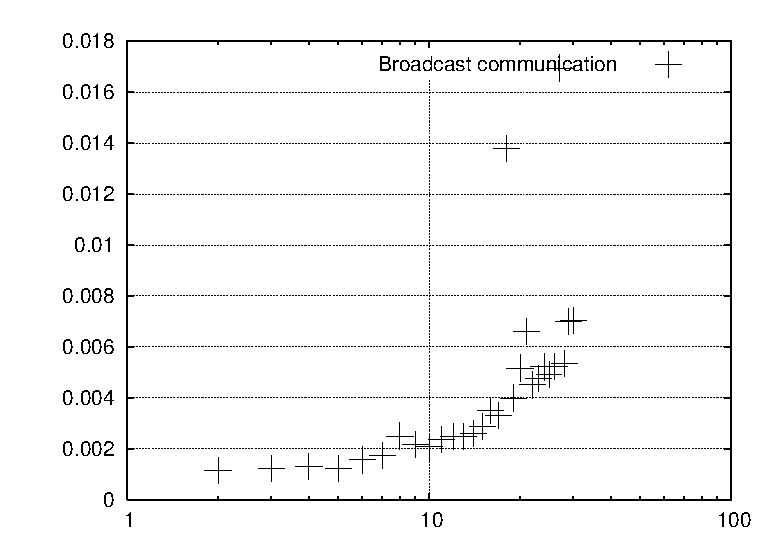
\includegraphics{bcast1.eps}

			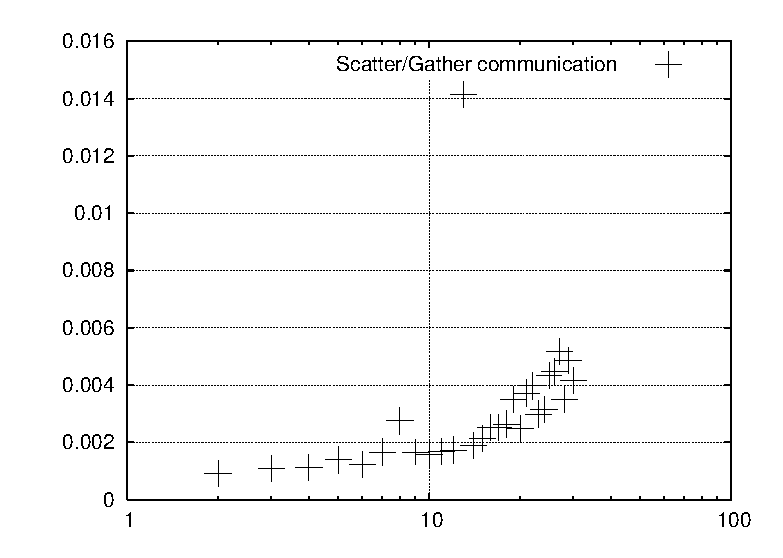
\includegraphics{scatter1.eps}

		\subsection{Topologia grafowa}
			W zadaniu nale�a�o stworzy� topologi� grafu i nast�pnie stworzy� co� na wz�r broadcastu. Nast�pnie nale�a�o sprawdzi� jak czas przesy�u zale�y od wielko�ci wiadomo�ci:

			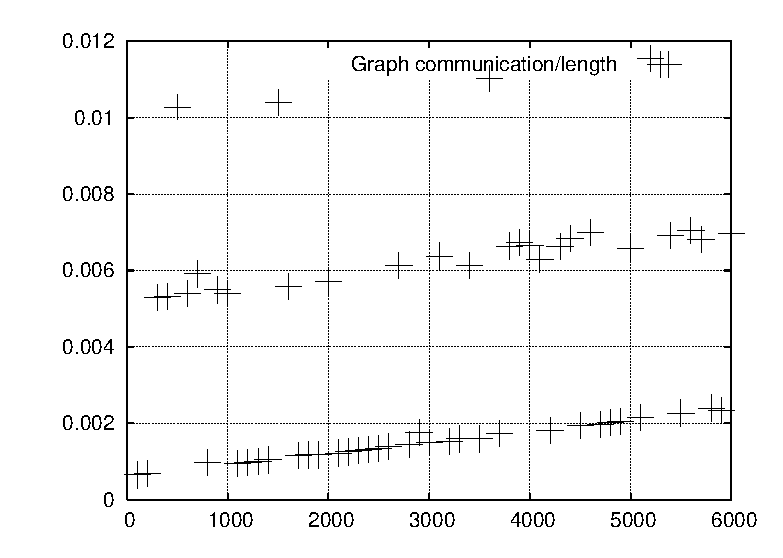
\includegraphics{len.eps}

			oraz jak spos�b grafowy r�ni si� od sposobu broadcastowego:

			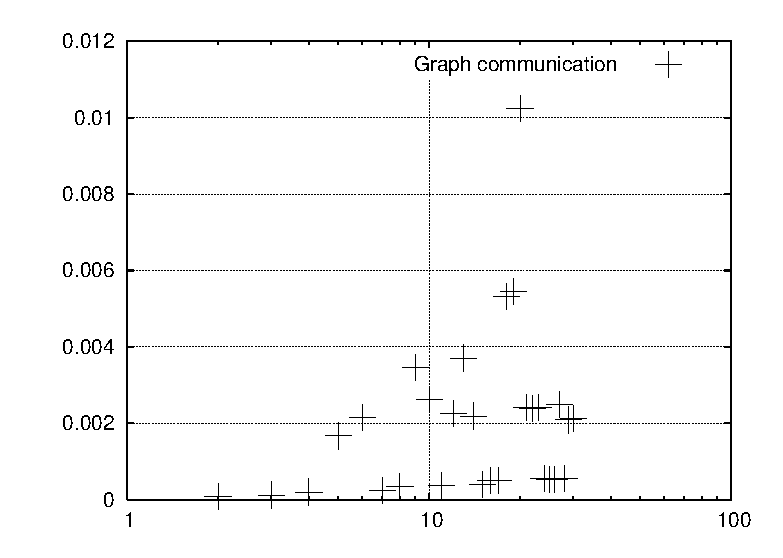
\includegraphics{graph.eps}

			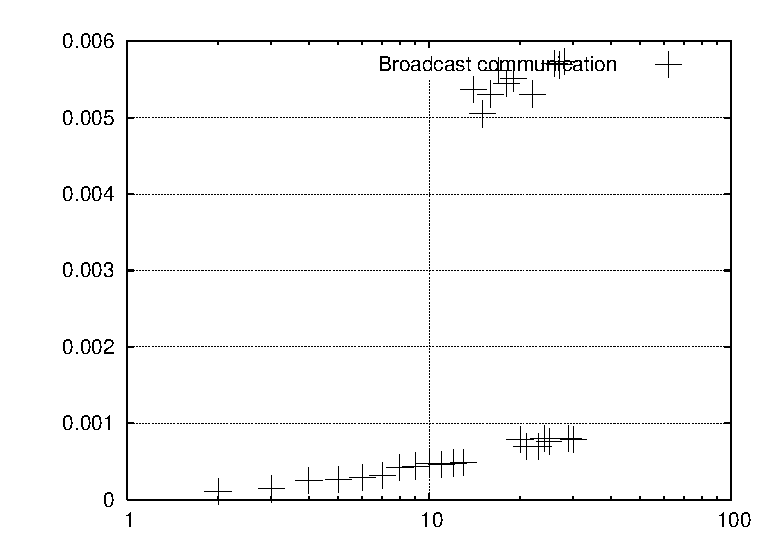
\includegraphics{bcast2.eps}

\end{document}
